\chapter{Μέθοδος Ελαχίστων Τετραγώνων}
Η μέθοδος ελαχίστων τετραγώνων για ευθεία γραμμή είναι μέθοδος εύρεσης την ευθείας με την ελάχιστη τετραγωνική απόσταση από τα δεδομένα. Αν έχουμε ένα σύνολο δεδομένων $(x_i,y_i),i-0,1,....n$
όπου τα $x_i$ θεωρούνται η ανεξάρτητη μεταβλητή. Ο σκοπός μας είναι να υπολογίσουμε τις παραμέτρους της ευθείας $y = m x+c$ έτσι ώστε να το άθροισμα των τετραγωνικών αποστάσεων των δεδομένων από την ευθεία να είναι ελαχιστοποιημένο. Η απόσταση ενός σημείου από την ευθεία είναι:
\begin{equation}
r_i = y_i-mx_i-c
\end{equation}
Αυτή η συνάρτηση δίνει την απόσταση της τιμής των δεδομένων από την ευθεία πρόβλεψης. Συνεπώς η ελαχιστοποίηση πρέπει να γίνει στην:
\begin{equation}
S=\sum_{i=1}^n r_i^2
\end{equation}
Πως χρησιμοποιούμε την {\en numpy} για την ευθεία ελαχίστων τετραγώνων:
\en
\begin{python}
import numpy.linalg as lin
import numpy as np

# data
x = np.array([0, 1, 2, 3])
y = np.array([-1, 0.2, 0.9, 2.1])

# we rewrite the equation as y=Ap where A=[[x 1]],p=[[m],[c]]
A = np.vstack([x, np.ones(len(x))]).T

# we put it in the function
m, c = lin.lstsq(A, y, rcond=None)[0]
m = round(m,3)
c = round(c,3)
m,c
\end{python}
\vspace*{-0.7cm}
\begin{codeout}
(1.0, -0.95)
\end{codeout}
\gr
Ας σχεδιάσουμε για να πάρουμε μία ιδέα για την ευθεία του παραδείγματος:
\en
\begin{python}
import matplotlib.pyplot as plt
_ = plt.plot(x, y, 'o', label='Original data', markersize=10)
_ = plt.plot(x, m*x + c, 'r', label='Fitted line')
_ = plt.legend()
plt.show()
\end{python}

\begin{center}
\begin{figure}[H]
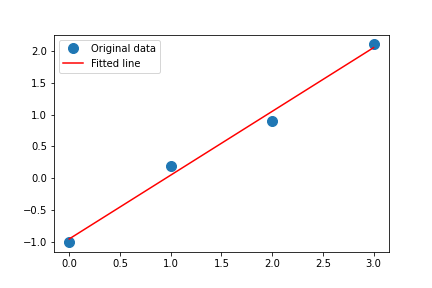
\includegraphics[scale=1]{figures/lsplot.png}
\end{figure}
\end{center}